\chapter{Anexo 4. Análisis contrafactual. Considera estrés térmico de 1989.}
\label{chap:anexo4}

Como complemento al análisis contrafactual desarrollado en la sección N°\ref{chap:contrafactual}, se replica el ejercicio de estimación, pero esta vez considerando la exposición al calor del año 1989, en lugar del promedio observado en el período 1970-1989. Esto, a fin de estudiar la sensibilidad de los resultados a un cambio en el horizonte temporal de referencia.

En este caso, entonces, se estudia un cambio en la tendencia del estrés térmico a partir del año 1990, con respecto al año inmediatamente anterior. Los principales resultados varían razonablemente. En principio, no debiera sorprender que existan variaciones con respecto al análisis revisado en el informe, ya que el principal motor del cambio es la temperatura de cada país, la que puede ser diferente según si se considera el promedio de una década o un año en específico.

Con todo, la principal discrepancia radica en la Tabla N°\ref{tab:surplus_1989}, donde se observa que el incremento del excedente de los líderes en el contrafactual es superior al de los seguidores. Dicho de otro modo, el estrés térmico en el factual habría perjudicado más a los líderes del mercado.

La Tabla N°\ref{tab:descomp_g_1989} reafirma estos resultados, y presenta la descomposición del efecto agregado entre sus componentes de eficiencia y estratégico. Se observa que el efecto estratégico para los seguidores es más relevante, lo que determina el resultado final.

\begin{table}[H]
\centering
\caption{Estimación de un escenario sin estrés térmico. Resultados de precios y cantidades.}
\label{tab:results_1989}
\begin{tabular}{lcc}
\hline
\textbf{Escenario} &
  \textbf{\begin{tabular}[c]{@{}c@{}}Precio promedio\\ (¢)\end{tabular}} &
  \textbf{\begin{tabular}[c]{@{}c@{}}Cantidad anual promedio\\ (mill. 60 kg.)\end{tabular}} \\ \hline
Factual &
  138 &
  92,8\\
Contrafactual &
  129 ($\downarrow$ 6,5\%) &
  93,3 ($\uparrow$ 0,5\%) \\ \hline
\end{tabular}%
\end{table}

\begin{table}[H]
\centering
\caption{Estimación de un escenario sin estrés térmico. Resultados de excedente social.}
\label{tab:surplus_1989}
\resizebox{\textwidth}{!}{
\begin{tabular}{lcccc}
\hline
\textbf{Escenario} &
  \textbf{\begin{tabular}[c]{@{}c@{}}Excedente\\ líderes \\ (mill. USD)\end{tabular}} &
  \textbf{\begin{tabular}[c]{@{}c@{}}Excedente\\ seguidores\\ (mill. USD)\end{tabular}} &
  \textbf{\begin{tabular}[c]{@{}c@{}}Excedente\\ importadores\\ (mill. USD)\end{tabular}} &
  \textbf{\begin{tabular}[c]{@{}c@{}}Excedente\\ total\\ (mill. USD)\end{tabular}} \\ \hline
Factual &
  37 &
  165 &
  10.124 &
  10.326 \\
Contrafactual &
  43,5 ($\uparrow$ 17,6\%) &
  145,6 ($\uparrow$ 11,8\%) &
  10.240 ($\uparrow$ 1\%) &
  10.429 ($\uparrow$ 1\%)  \\ \hline
\end{tabular}
}
\end{table}

% Please add the following required packages to your document preamble:
% \usepackage{graphicx}
\begin{table}[H]
\centering
\caption{Descomposición del excedente total acumulado en 1990-2019 (mill. USD)}
\label{tab:descomp_g_1989}
\begin{tabular}{lccc}
\hline
            & \textbf{Efecto eficiencia} & \textbf{Efecto estratégico} & \textbf{Efecto total} \\ \hline
Líderes     & 1.421             & -1.239             & 181          \\
Seguidores  & 1.506             & -2.052             & -545        \\ \hline
\end{tabular}%

\end{table}

Por último, tanto las Figuras N°\ref{fig:diff_profit_2} y \ref{fig:diff_profit_2}, como las Figuras N°\ref{fig:descomp_c_1989} y \ref{fig:descomp_c_2} muestran claramente una estabilidad del patrón en el cambio del beneficio por país y en la descomposición del efecto neto del cambio en el estrés térmico. Esto, a pesar de que exista una diferencia en niveles, que explica los cambios en los demás resultados analizados.

\begin{figure}[H]
    \centering
    \caption{Cambio en el beneficio por país. Comparación con 1989}
        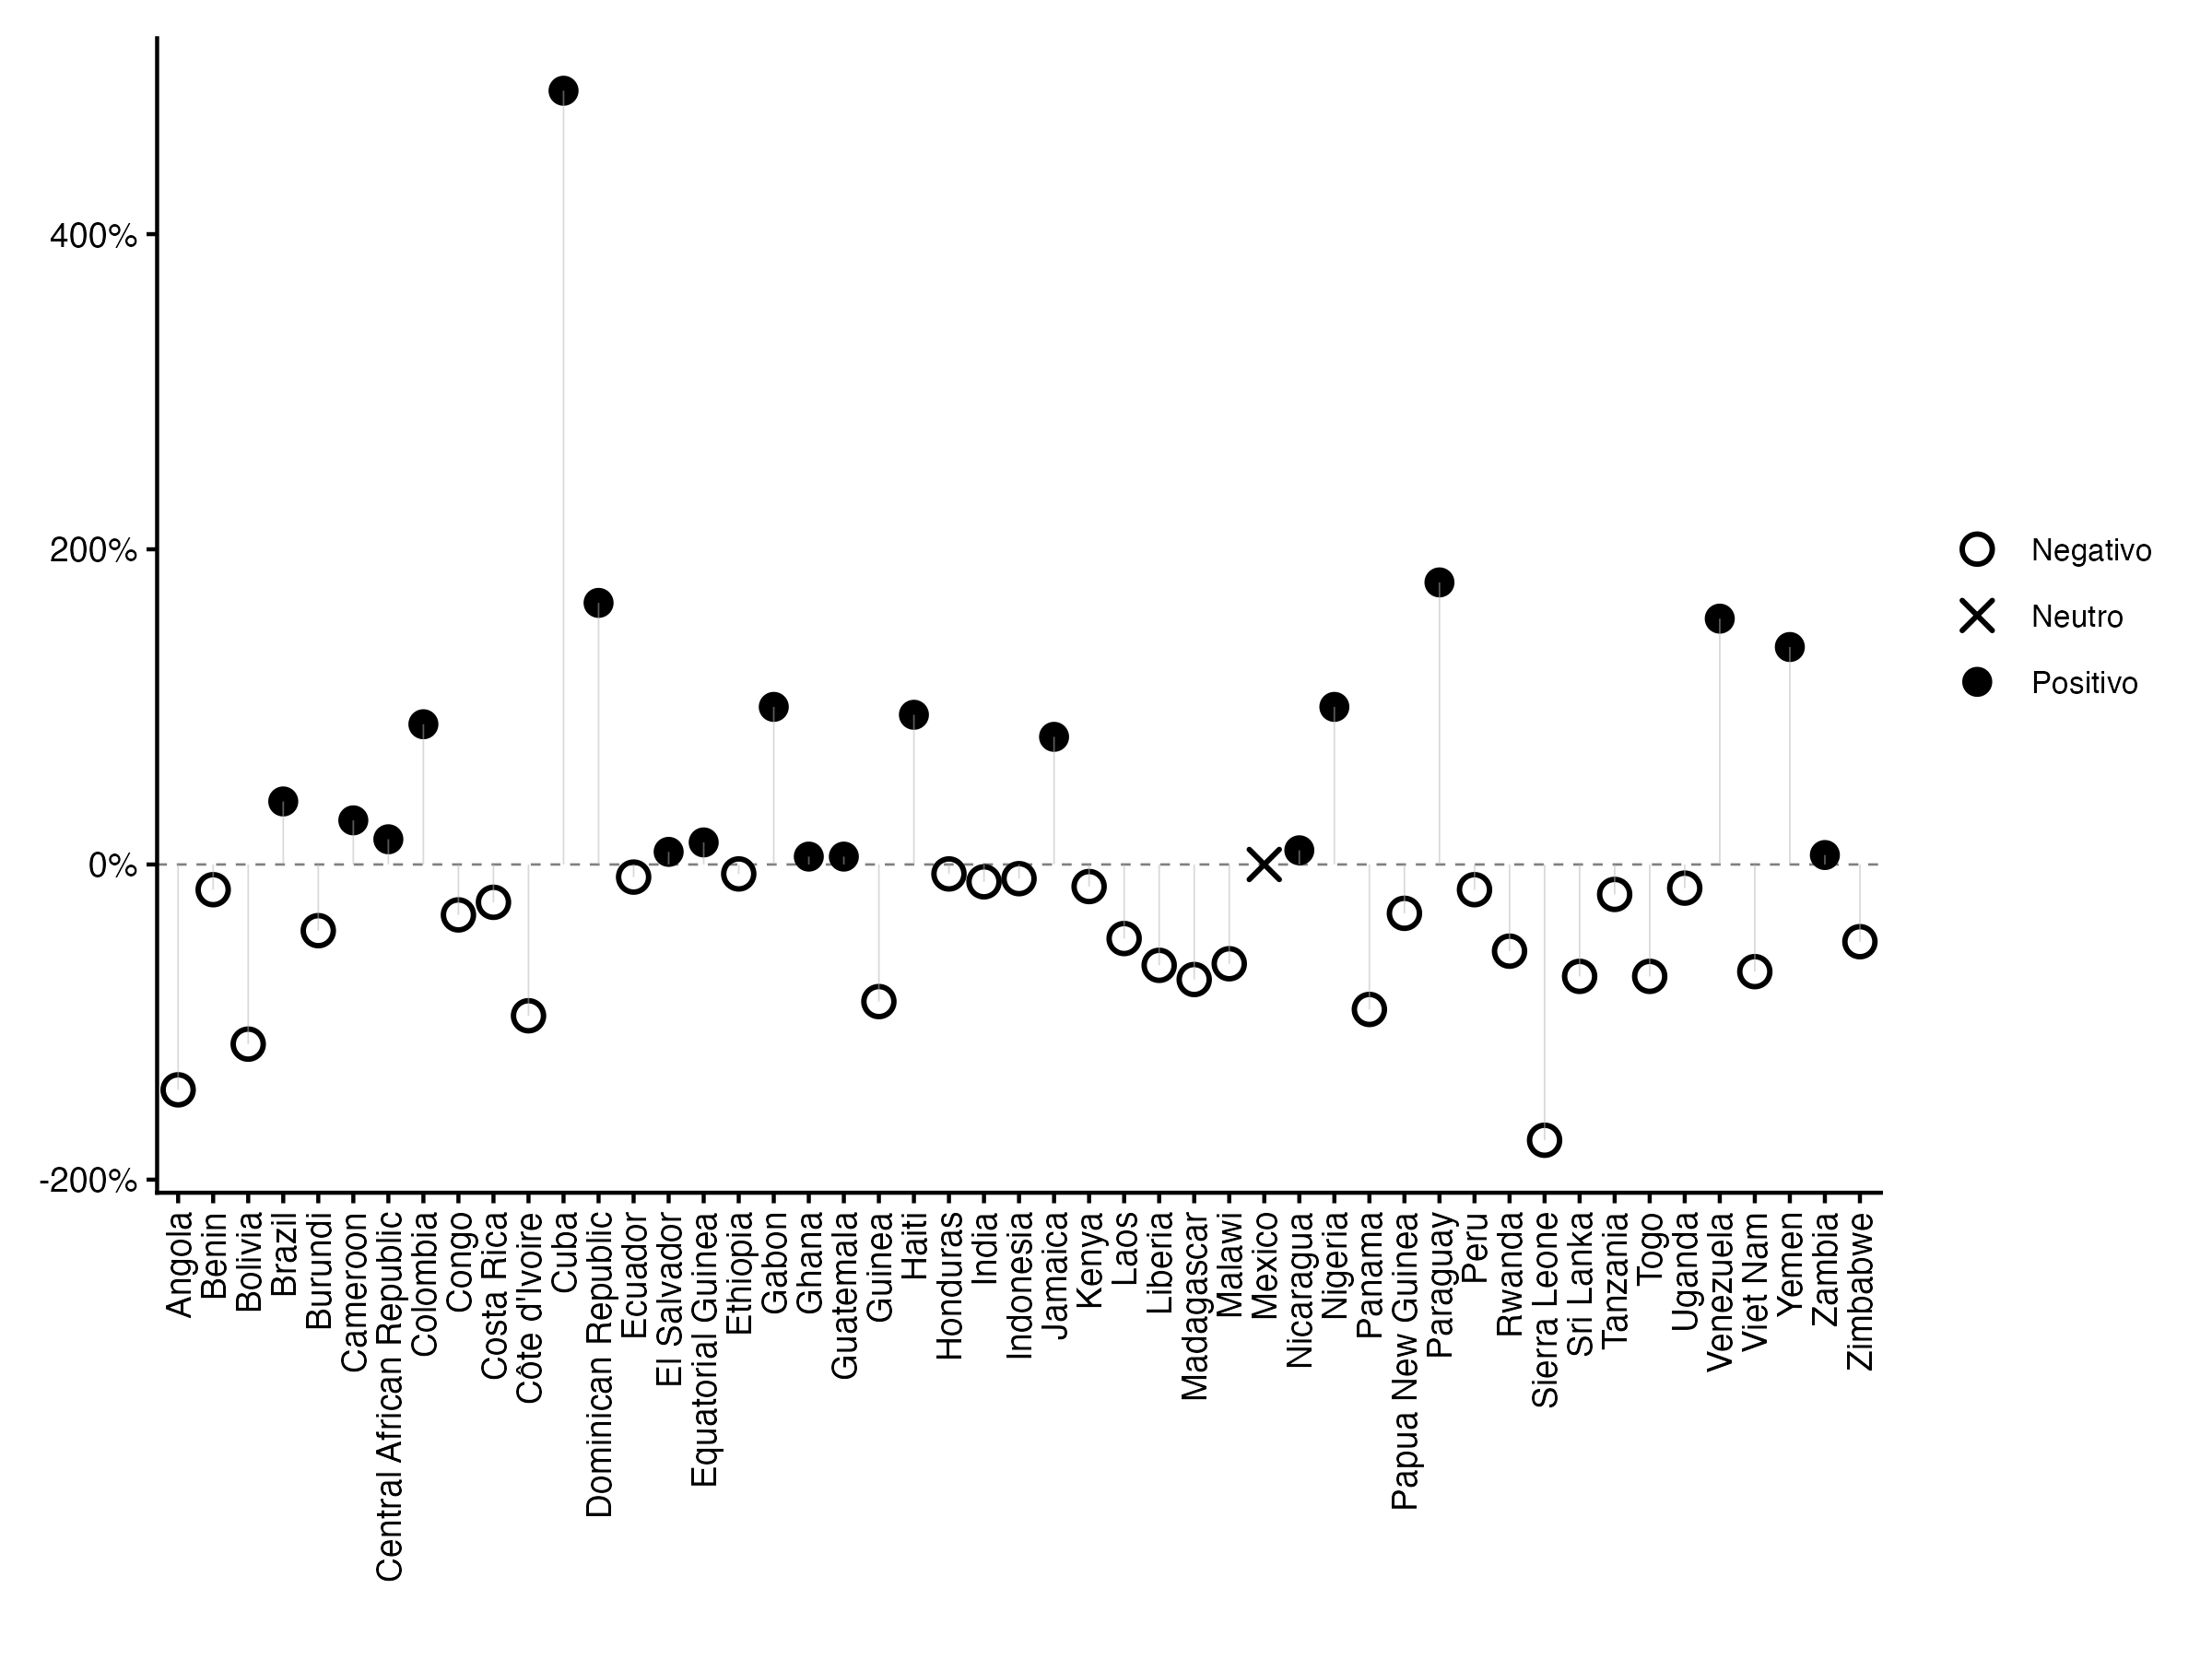
\includegraphics[scale = 0.6]{figures/diff_profit_1989.png}
        \label{fig:diff_profit_1989}
\end{figure}

\begin{figure}[H]
    \centering
    \caption{Cambio en el beneficio por país. Comparación con 1970-1989}
        
\includegraphics[scale = 0.6]{figures/diff_profit.png}
        \label{fig:diff_profit_2}
\end{figure}

\begin{figure}[H]
    \centering
    \caption{Descomposición del excedente total acumulado en 1990-2019, por país. Comparación con 1989}
        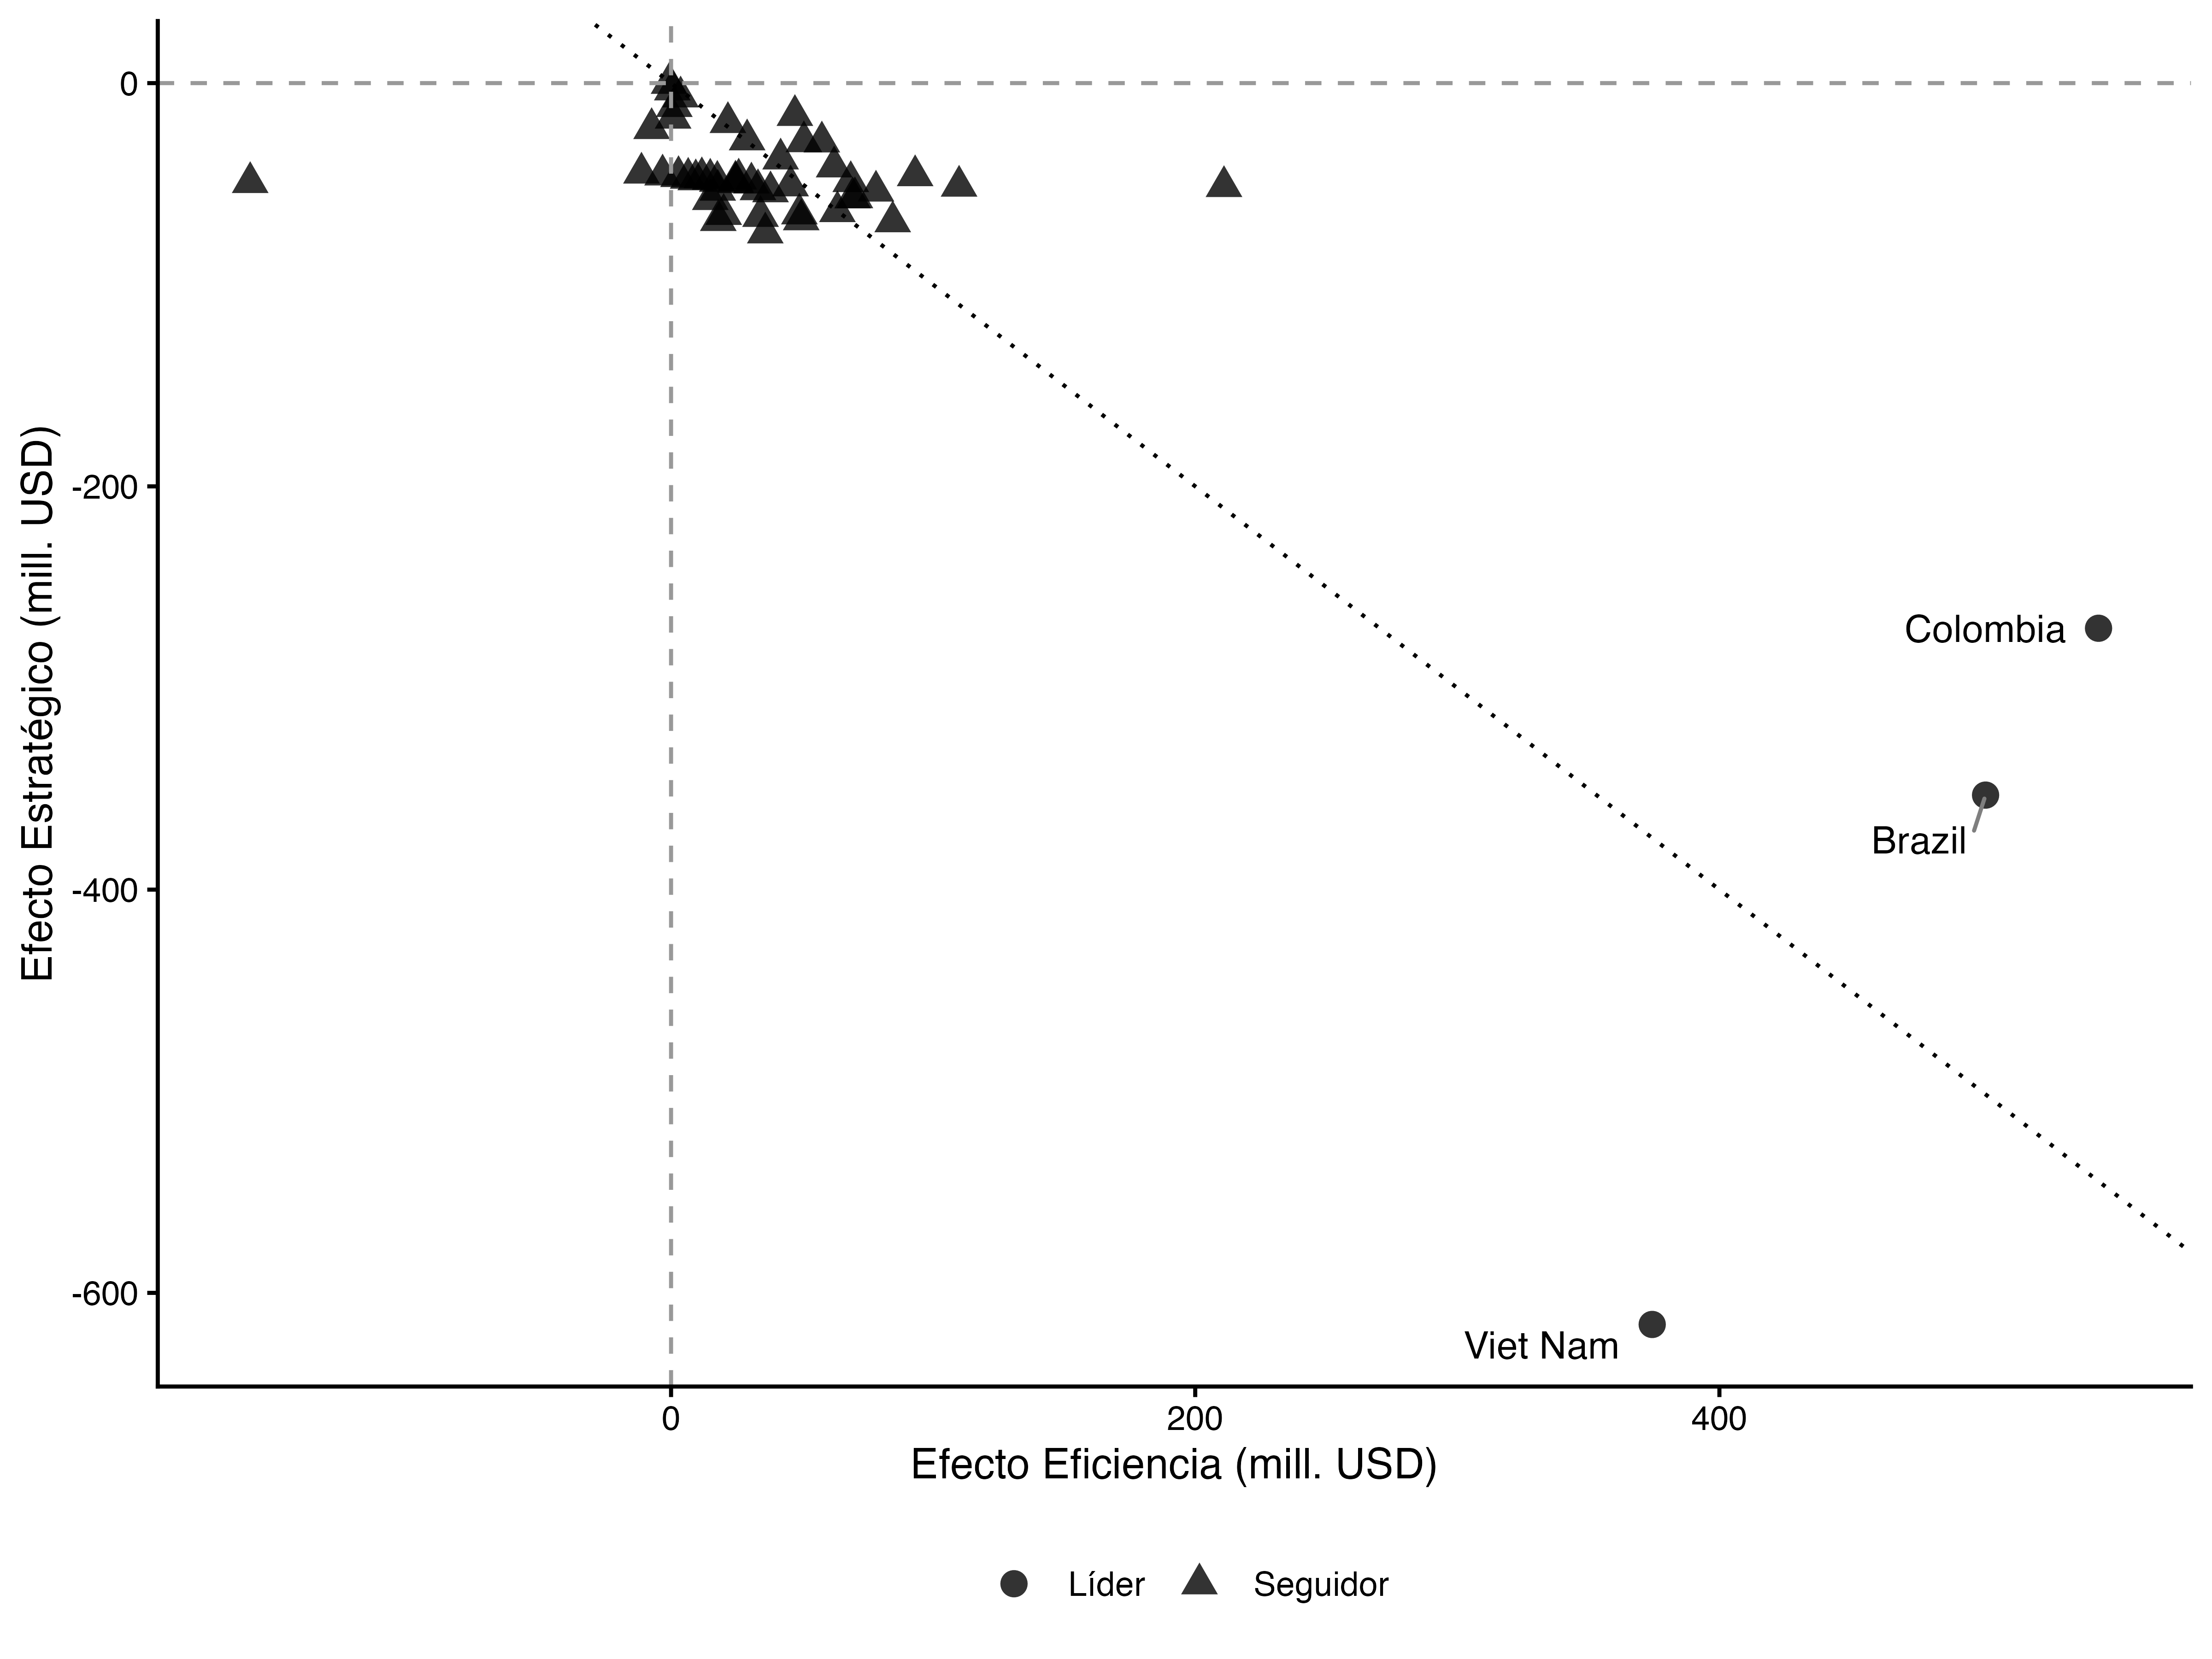
\includegraphics[scale = 0.6]{figures/plot_descomp_c_1989}
        \label{fig:descomp_c_1989}
\end{figure}

\begin{figure}[H]
    \centering
    \caption{Descomposición del excedente total acumulado en 1990-2019, por país. Comparación con 1970-1989}
        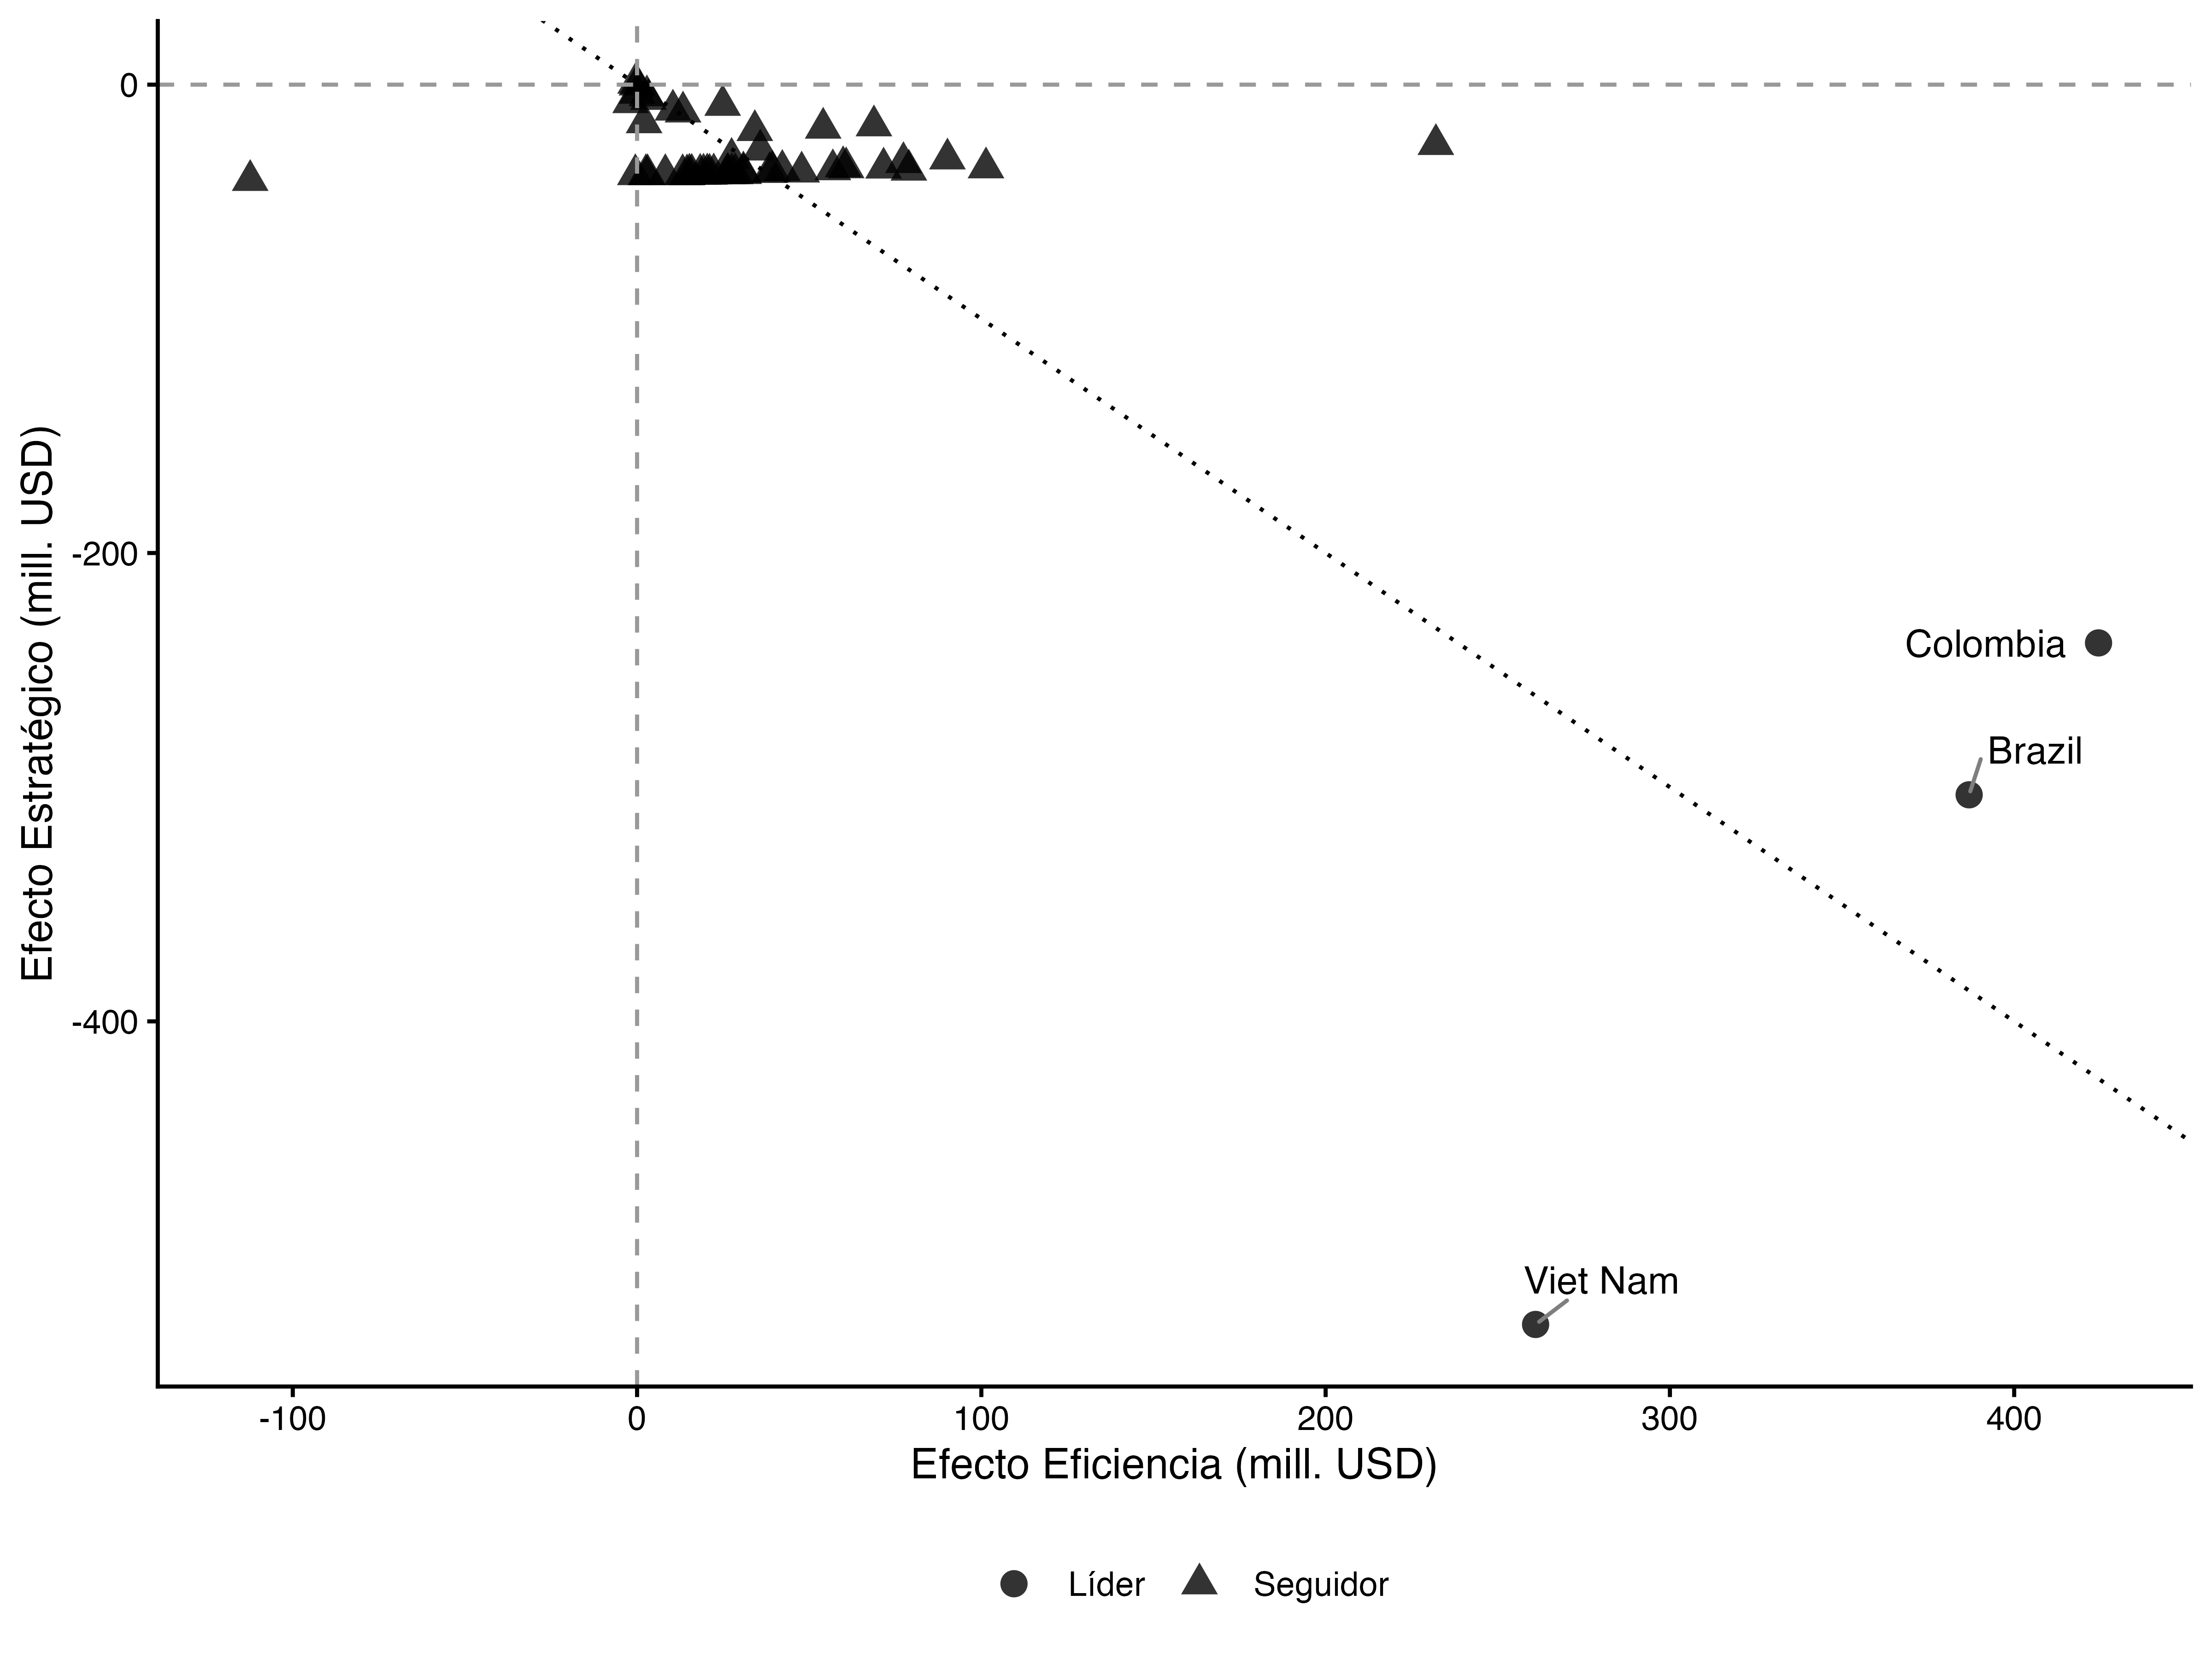
\includegraphics[scale = 0.6]{figures/plot_descomp_c}
        \label{fig:descomp_c_2}
\end{figure}
